% ============================================================
% Evaluación 04 — Reporte: Curso "Conceptos Básicos de Redes"
% Cisco Networking Academy · Habilidades para Todos
% Redes de Comunicaciones de Datos (6.º semestre)
% UAZ · Unidad Académica de Ingeniería Eléctrica
% ============================================================
\documentclass[11pt,a4paper]{article}

\usepackage[utf8]{inputenc}
\usepackage[T1]{fontenc}
\usepackage[spanish,mexico]{babel}
\usepackage{graphicx}
\usepackage[margin=2.5cm]{geometry}
\usepackage{setspace}
\usepackage{parskip}
\usepackage{fancyhdr}
\usepackage{pdfpages}
\usepackage{xcolor}
\usepackage{booktabs}
\usepackage[hidelinks]{hyperref}
\usepackage{xurl}
\usepackage{enumitem}

\onehalfspacing
\setlength{\parskip}{6pt}

% Marcador visible para evidencia que todavía falta capturar.
% Se borra cuando la figura real está incluida.
\newcommand{\pendiente}[1]{\textcolor{red}{\textbf{[PENDIENTE: #1]}}}

\setlength{\headheight}{40pt}
\pagestyle{fancy}
\fancyhf{}
\fancyhead[L]{
\includegraphics[width=1cm]{../../../Assets/UIE.png}}
\fancyfoot[C]{\thepage}
\renewcommand{\headrulewidth}{0.4pt}

\begin{document}

% ---------------------------- PORTADA -----------------------
\begin{titlepage}
  \thispagestyle{empty}
  \begin{center}
    \vspace*{1cm}
    
\includegraphics[width=4.5cm]{../../../Assets/uaz.png}
    \vspace{0.8cm}

    {\large Universidad Autónoma de Zacatecas}\\[4pt]
    {\large Unidad Académica de Ingeniería Eléctrica}\\[4pt]
    {\normalsize Ingeniería Electrónica Industrial con especialidad en Telecomunicaciones}

    \vspace{1.8cm}
    {\LARGE\bfseries Evaluación 04}\\[10pt]
    {\Large\bfseries Reporte de finalización del curso:\\[4pt]
     Conceptos Básicos de Redes}
  \end{center}

  \vspace{2.2cm}
  \begin{center}
    \begin{tabular}{rl}
      \textbf{Materia:} & Redes de Comunicaciones de Datos\\
      \textbf{Docente:} & José Ricardo Gómez Rodríguez\\
      \textbf{Alumno:}  & Arnold Yovick Ríos Zaldívar\\
      \textbf{Fecha:}   & Noviembre de 2026\\
    \end{tabular}
  \end{center}
  \vfill
\end{titlepage}

% ------------------------- INTRODUCCIÓN ---------------------
\section{Introducción}

El curso \textit{Conceptos Básicos de Redes} (\textit{Networking Basics})
de Cisco Networking Academy, ofrecido a través de la plataforma Habilidades
para Todos, constituye el punto de partida de la formación en redes de datos.
Su propósito es consolidar los fundamentos sobre los que se construyen las
tecnologías de comunicación: los modelos de referencia OSI y TCP/IP, los tipos
de red (LAN, WAN y WLAN), los dispositivos que intervienen en una
infraestructura (switch, router, firewall, punto de acceso), los medios de
transmisión y el direccionamiento IP, junto con los protocolos de comunicación
de mayor uso.

A diferencia de un curso centrado en un simulador, este curso construye el
marco conceptual: explica \emph{por qué} una red funciona antes de explicar
\emph{cómo} configurarla. Esa es precisamente la base que la materia de Redes
de Comunicaciones de Datos requiere para abordar después el enrutamiento, la
conmutación y el diseño de infraestructuras de mayor complejidad.

El curso se organiza en diecisiete módulos agrupados en cuatro bloques
temáticos, intercalados con exámenes de punto de control que verifican la
comprensión acumulada, y culmina con un examen final. A lo largo del recorrido
se realizan actividades interactivas, cuestionarios y simulaciones en Cisco
Packet Tracer que permiten aplicar los conceptos teóricos en escenarios
prácticos.

El presente reporte documenta el recorrido completo del curso, sintetiza los
contenidos de cada bloque temático, explica el comportamiento de los paquetes
y la interacción entre los modelos OSI y TCP/IP, y presenta las evidencias de
finalización: la constancia del progreso al 100\,\% y el certificado emitido
por Cisco Networking Academy (Anexo~A).

% -------------------------- OBJETIVOS -----------------------
\section{Objetivos}

\subsection{Objetivo general}

Completar el curso \textit{Conceptos Básicos de Redes} de Cisco Networking
Academy, consolidando los conocimientos fundamentales sobre redes de datos y
demostrando su aplicación mediante la simulación de topologías en Cisco Packet
Tracer.

\subsection{Objetivos específicos}

\begin{itemize}[leftmargin=*]
  \item Describir los modelos de referencia OSI y TCP/IP e identificar la
        función de cada una de sus capas.
  \item Distinguir los tipos de red (LAN, WAN y WLAN) y los dispositivos que
        intervienen en cada uno de ellos.
  \item Identificar los medios de transmisión y las características que
        determinan su elección en un diseño de red.
  \item Aplicar el direccionamiento IPv4 e IPv6, incluyendo la segmentación
        de redes y el direccionamiento dinámico mediante DHCP.
  \item Explicar el funcionamiento del proceso ARP y su papel en la entrega
        de tramas dentro de una LAN.
  \item Comparar el comportamiento de los protocolos de transporte TCP y UDP
        y justificar su uso según el tipo de aplicación.
  \item Analizar, con apoyo de Cisco Packet Tracer, el flujo de un paquete a
        través de la red y su correspondencia con las capas de los modelos.
  \item Emplear utilidades de prueba de red para diagnosticar problemas de
        conectividad.
\end{itemize}

% -------------------------- DESARROLLO ----------------------
\section{Desarrollo}

\subsection{Panorama y estructura del curso}

El curso se distribuye en diecisiete módulos que avanzan de lo general a lo
particular. Los cuatro primeros describen el panorama de las redes y el
funcionamiento de una red doméstica; el quinto establece los principios de
comunicación; los módulos sexto y séptimo descienden al medio físico y a la
capa de acceso; del octavo al decimocuarto se concentra el direccionamiento y
el enrutamiento; y los tres últimos cubren el transporte, los servicios de
aplicación y las herramientas de diagnóstico.

\begin{table}[htbp]
  \centering
  \small
  \begin{tabular}{@{}cl@{}}
    \toprule
    \textbf{Bloque} & \textbf{Módulos} \\ \midrule
    Panorama de las redes & 1. Comunicación en un mundo conectado \\
                          & 2. Componentes, tipos y conexiones de red \\
                          & 3. Redes inalámbricas y móviles \\
                          & 4. Crear una red doméstica \\ \addlinespace
    Principios y medios   & 5. Principios de comunicación \\
                          & 6. Medios de red \\
                          & 7. La capa de acceso \\ \addlinespace
    Direccionamiento y enrutamiento
                          & 8. El Protocolo de Internet \\
                          & 9. IPv4 y segmentación de redes \\
                          & 10. Formatos y reglas de IPv6 \\
                          & 11. Direccionamiento dinámico con DHCP \\
                          & 12. Puertas de enlace a otras redes \\
                          & 13. El proceso ARP \\
                          & 14. Enrutamiento entre redes \\ \addlinespace
    Transporte y servicios
                          & 15. TCP y UDP \\
                          & 16. Servicios de la capa de aplicación \\
                          & 17. Utilidades de prueba de red \\ \bottomrule
  \end{tabular}
  \caption{Organización temática de los diecisiete módulos del curso.}
  \label{tab:estructura}
\end{table}

\subsection{Comunicación en un mundo conectado}

El primer módulo establece por qué las redes importan: permiten compartir
recursos, acceder a información distribuida y sostener servicios que van desde
la mensajería hasta la administración remota de infraestructura. Se introducen
los conceptos de red, de host y de medio, así como las distintas escalas de
interconexión: desde una red personal hasta Internet como red de redes.

Un punto central del módulo es la distinción entre la red como
\emph{infraestructura} (dispositivos y medios) y la red como
\emph{servicio} (lo que el usuario percibe). Esta separación explica por qué
un diagnóstico debe empezar por verificar la capa física antes de suponer una
falla en la aplicación.

\subsection{Componentes, tipos y conexiones de red}

Aquí se clasifican los elementos de una red en tres grupos: \textbf{equipos
finales} (computadoras, servidores, teléfonos, impresoras), \textbf{dispositivos
intermedios} (switch, router, punto de acceso, firewall) y \textbf{medios}
(cobre, fibra óptica, radiofrecuencia).

Los tipos de red se distinguen por alcance y propósito:

\begin{itemize}[leftmargin=*]
  \item \textbf{LAN} (\textit{Local Area Network}): red de área local, de
        extensión limitada a un edificio o campus, caracterizada por altas
        velocidades y administración de un solo dominio.
  \item \textbf{WAN} (\textit{Wide Area Network}): red de área amplia, que
        interconecta sedes geográficamente distantes mediante enlaces
        provistos por un operador. Internet es la WAN más grande.
  \item \textbf{WLAN} (\textit{Wireless LAN}): LAN implementada con medios
        inalámbricos, que agrega movilidad a costa de compartir un medio
        común y requerir mecanismos de seguridad adicionales.
\end{itemize}

Cada dispositivo cumple una función delimitada: el \textbf{switch} conmuta
tramas dentro de una LAN a partir de direcciones MAC; el \textbf{router}
interconecta redes distintas y decide la ruta de los paquetes a partir de
direcciones IP; el \textbf{firewall} filtra el tráfico según reglas de
seguridad; y el \textbf{punto de acceso} extiende la LAN a los clientes
inalámbricos.

\subsection{Redes inalámbricas y móviles}

El módulo sobre redes inalámbricas aborda la transmisión por radiofrecuencia,
sus ventajas (movilidad, costo de instalación) y sus limitaciones
(interferencia, atenuación, compartición del medio). Se estudian los
estándares de la familia IEEE 802.11, las bandas de frecuencia empleadas y la
incidencia del entorno físico en la cobertura.

También se cubren las redes móviles y el concepto de anclaje
(\textit{tethering}), que permite compartir la conexión celular de un
dispositivo con otros equipos, así como las consideraciones de seguridad
inherentes a las redes inalámbricas abiertas: el tráfico comparte un medio
que no está confinado al edificio, por lo que el cifrado deja de ser opcional.

\subsection{Crear una red doméstica}

Este bloque aplica los conceptos anteriores a un escenario concreto: la red de
una vivienda. Se revisa el papel del router inalámbrico integrado, que combina
las funciones de router, switch y punto de acceso, y se describen las tareas de
puesta en marcha: conexión del módem, configuración de la red inalámbrica,
elección del canal, establecimiento de la contraseña y verificación de la
conectividad de los equipos finales.

Se introduce además el direccionamiento privado asignado por DHCP dentro de la
red doméstica y el mecanismo de traducción de direcciones que permite que
varios dispositivos compartan una única dirección pública, tema que se retoma
con profundidad en el módulo~12.

\subsection{Principios de comunicación: protocolos, estándares y modelos}

Este es el módulo que estructura conceptualmente todo el curso. Un
\textbf{protocolo} es un conjunto de reglas que gobierna el intercambio de
mensajes: define el método de comunicación, el formato o codificación de los
datos, el tamaño de los mensajes, la temporización y las estrategias de
confirmación y recuperación ante errores. Sin reglas compartidas no hay
comunicación posible, del mismo modo que dos personas necesitan un idioma
común y un turno de palabra.

Los \textbf{estándares} garantizan que equipos de fabricantes distintos puedan
interoperar. Los principales organismos son IEEE (estándares de LAN, como
802.3 Ethernet y 802.11 inalámbrico), IETF (protocolos de Internet, publicados
como RFC) e ISO (modelo de referencia OSI).

\paragraph{Modelo OSI.} Divide la comunicación en siete capas, cada una con una
responsabilidad definida:

\begin{enumerate}[leftmargin=*]
  \item \textbf{Física}: transmisión de bits por el medio.
  \item \textbf{Enlace de datos}: entrega de tramas entre nodos adyacentes,
        con direccionamiento MAC y detección de errores.
  \item \textbf{Red}: direccionamiento lógico y determinación de la ruta.
  \item \textbf{Transporte}: segmentación, control de flujo y confiabilidad
        extremo a extremo.
  \item \textbf{Sesión}: establecimiento, mantenimiento y cierre de diálogos.
  \item \textbf{Presentación}: formato, compresión y cifrado de los datos.
  \item \textbf{Aplicación}: interfaz con los servicios de usuario.
\end{enumerate}

\paragraph{Modelo TCP/IP.} Es el modelo efectivamente implementado y consta de
cuatro capas: acceso a la red (equivalente a física y enlace de OSI),
Internet (equivalente a red), transporte y aplicación (que agrupa sesión,
presentación y aplicación). La Tabla~\ref{tab:osi-tcpip} resume la
correspondencia.

\begin{table}[htbp]
  \centering
  \small
  \begin{tabular}{@{}p{3.1cm}p{2.6cm}p{6.4cm}@{}}
    \toprule
    \textbf{OSI} & \textbf{TCP/IP} & \textbf{Protocolos representativos} \\ \midrule
    Aplicación, Presentación, Sesión & Aplicación & HTTP, HTTPS, DNS, DHCP, FTP, SMTP, IMAP, SSH \\
    Transporte & Transporte & TCP, UDP \\
    Red & Internet & IPv4, IPv6, ICMP, ARP \\
    Enlace de datos & Acceso a la red & Ethernet (802.3), Wi-Fi (802.11) \\
    Física & Acceso a la red & Cobre UTP, fibra óptica, radiofrecuencia \\ \bottomrule
  \end{tabular}
  \caption{Correspondencia entre las capas de los modelos OSI y TCP/IP, con los
  protocolos representativos de cada nivel.}
  \label{tab:osi-tcpip}
\end{table}

La utilidad práctica de esta distinción es diagnóstica: el modelo OSI es una
referencia que permite localizar en qué nivel ocurre una falla. Un cable
desconectado es un problema de capa~1; una MAC equivocada, de capa~2; una
dirección IP fuera de rango, de capa~3; un puerto cerrado, de capa~4; y un
error de configuración en el servicio, de capa~7.

\subsection{Medios de red y capa de acceso}

El módulo~6 clasifica los medios de transmisión. El \textbf{cable de par
trenzado} (UTP) es el más difundido en LAN: categorías como Cat5e, Cat6 y Cat6a
determinan el ancho de banda soportado y la inmunidad al ruido. La
\textbf{fibra óptica} transporta información mediante luz, ofrece mayor
alcance y capacidad, y es inmune a la interferencia electromagnética, lo que
la hace idónea para enlaces troncales y distancias largas. El medio
\textbf{inalámbrico} prescinde del cable pero comparte un espectro limitado.

El módulo~7 estudia la capa de acceso, donde opera Ethernet. Se describen las
funciones del switch: aprendizaje de direcciones MAC a partir de la dirección
de origen de las tramas recibidas, construcción de su tabla de conmutación,
reenvío selectivo por el puerto correspondiente, inundación
(\textit{flooding}) cuando el destino es desconocido y descarte de tramas
cuando origen y destino comparten puerto. Se introduce también la diferencia
entre dominio de colisión y dominio de difusión, y el papel de la VLAN como
segmentación lógica.

\subsection{Direccionamiento IP: IPv4, segmentación e IPv6}

\paragraph{IPv4.} Una dirección IPv4 es un número de 32 bits (cuatro octetos)
que identifica de forma lógica una interfaz. Se compone de una porción de red y
una porción de host, delimitadas por la máscara de subred. Las direcciones se
clasifican en públicas y privadas; los rangos privados definidos en la RFC 1918
son \texttt{10.0.0.0/8}, \texttt{172.16.0.0/12} y \texttt{192.168.0.0/16}, y no
se enrutan en Internet.

\paragraph{Segmentación.} La división en subredes permite partir un bloque de
direcciones en redes más pequeñas y administrables, mejorando la seguridad y
reduciendo el dominio de difusión. Conceptos clave: máscara de subred, prefijo
CIDR, dirección de red, dirección de difusión y número de hosts utilizables,
que para una subred de $n$ bits de host es $2^{n}-2$ (se excluyen la dirección
de red y la de difusión). Por ejemplo, \texttt{192.168.10.0/26} deja 6 bits de
host y por tanto $2^{6}-2 = 62$ direcciones utilizables.

\paragraph{IPv6.} El agotamiento del espacio de IPv4 motivó el diseño de IPv6,
con direcciones de 128 bits expresadas en ocho grupos hexadecimales. Se
abrevian omitiendo ceros iniciales y sustituyendo un único bloque contiguo de
grupos nulos por \texttt{::}. IPv6 elimina la necesidad de NAT, define tipos de
dirección (unidifusión, multidifusión y \textit{anycast}), incorpora
autoconfiguración y simplifica la cabecera para agilizar el reenvío.

\subsection{Direccionamiento dinámico con DHCP}

Asignar direcciones manualmente no escala. DHCP (\textit{Dynamic Host
Configuration Protocol}) automatiza el proceso mediante cuatro mensajes:

\begin{enumerate}[leftmargin=*]
  \item \textbf{DHCPDISCOVER}: el cliente difunde la búsqueda de un servidor
        DHCP, pues aún no posee dirección y no puede ser direccionado.
  \item \textbf{DHCPOFFER}: el servidor responde ofreciendo una dirección
        disponible junto con la máscara, la puerta de enlace y el servidor DNS.
  \item \textbf{DHCPREQUEST}: el cliente solicita formalmente la dirección
        ofrecida.
  \item \textbf{DHCPACK}: el servidor confirma la asignación y fija el tiempo
        de concesión.
\end{enumerate}

Los tres primeros intercambios emplean difusión; el cuarto puede ser
unidifusión. La concesión (\textit{lease}) es temporal y se renueva, lo que
permite recuperar direcciones de equipos que abandonan la red. En una red
doméstica el router inalámbrico cumple la función de servidor DHCP.

\subsection{Puertas de enlace y traducción de direcciones}

La \textbf{puerta de enlace predeterminada} es la dirección del router de la
red local al que el host entrega los paquetes cuyo destino no pertenece a su
propia subred. Sin ella, el host solo puede comunicarse dentro de su dominio.

El módulo~12 estudia NAT (\textit{Network Address Translation}), que permite
que múltiples hosts con direcciones privadas compartan una dirección pública.
En su variante más común, PAT (\textit{Port Address Translation}), el router
sustituye la dirección privada de origen por la pública y asigna un puerto
distinto a cada conversación, manteniendo una tabla que le permite revertir la
traducción en el sentido de regreso. NAT resolvió la escasez de IPv4 a costa
de romper la conectividad extremo a extremo y complicar protocolos que
transportan direcciones dentro de la carga útil.

\subsection{El proceso ARP}

Dentro de una LAN, los datos viajan en tramas que se entregan por dirección
MAC, no por dirección IP. ARP (\textit{Address Resolution Protocol}) tiende el
puente entre ambos esquemas: cuando un host conoce la IP de destino pero no su
MAC, difunde una solicitud ARP (\textit{ARP request}) preguntando quién posee
esa dirección; el propietario responde con su MAC (\textit{ARP reply}), y el
solicitante guarda la correspondencia en su tabla ARP durante un tiempo
limitado.

Si el destino está en otra red, el host no resuelve la MAC del destino final
sino la de la puerta de enlace. Este detalle es el que explica un hecho
fundamental del reenvío: \textbf{las direcciones IP se conservan de extremo a
extremo, mientras que las direcciones MAC se reescriben en cada salto}.

\subsection{Enrutamiento entre redes}

El router decide por dónde enviar cada paquete consultando su tabla de
enrutamiento, que asocia redes de destino con la interfaz de salida o el
siguiente salto. La decisión sigue el principio de la coincidencia más
específica: se elige la ruta con el prefijo más largo que contenga la
dirección de destino. Cuando ninguna ruta coincide, se emplea la ruta
predeterminada (\texttt{0.0.0.0/0}), que apunta hacia el siguiente router.

Se revisan también las diferencias entre la configuración estática, adecuada
para redes pequeñas y estables, y el enrutamiento dinámico, en el que los
routers intercambian información mediante protocolos para adaptarse
automáticamente a cambios en la topología.

\subsection{TCP y UDP}

Ambos protocolos operan en la capa de transporte, pero con filosofías opuestas.

\textbf{TCP} es orientado a conexión y confiable: establece la sesión mediante
un saludo de tres vías (\textit{SYN}, \textit{SYN-ACK}, \textit{ACK}),
numera los segmentos, confirma su recepción, retransmite lo perdido y ordena
los datos en destino. Su costo es la sobrecarga de cabecera y de gestión. Se
emplea en aplicaciones donde la integridad es indispensable: HTTP, correo,
transferencia de archivos, SSH.

\textbf{UDP} no establece conexión ni garantiza entrega ni orden: simplemente
envía datagramas con un esfuerzo mínimo. Su ventaja es la baja latencia y la
ausencia de sobrecarga, lo que lo hace adecuado para transmisión en tiempo
real (voz, video), consultas DNS y protocolos de administración. La
confiabilidad, cuando se requiere, se delega en la aplicación.

\subsection{Servicios de la capa de aplicación}

El módulo~16 recorre los servicios que el usuario final utiliza y su
dependencia de la infraestructura subyacente. HTTP y HTTPS sostienen la web,
con HTTPS añadiendo cifrado mediante TLS. DNS traduce nombres de dominio a
direcciones IP y es condición previa a casi cualquier acceso. DHCP asigna
configuración de red. FTP transfiere archivos, mientras que SSH y Telnet
ofrecen administración remota, con la salvedad de que Telnet transmite en
claro y debe evitarse. Los servicios de correo (SMTP para envío, IMAP y POP
para recepción) ilustran cómo un mismo servicio se descompone en protocolos
distintos.

Un concepto que atraviesa el módulo es el de \textbf{puerto}: el número de
puerto identifica la aplicación dentro del host y permite que múltiples
servicios convivan en una misma dirección IP.

\subsection{Utilidades de prueba de red}

El último módulo presenta las herramientas de diagnóstico que permiten
convertir los conceptos anteriores en un procedimiento de verificación:

\begin{itemize}[leftmargin=*]
  \item \texttt{ipconfig}: muestra la configuración IP del host; con
        \texttt{/all} incluye MAC, servidores DHCP y DNS.
  \item \texttt{ping}: comprueba alcanzabilidad de capa~3 mediante mensajes
        ICMP y reporta el tiempo de ida y vuelta.
  \item \texttt{tracert}: revela la ruta hop a hop hasta el destino y permite
        localizar el punto donde se pierde la conectividad.
  \item \texttt{nslookup}: consulta la resolución de nombres contra el
        servidor DNS.
  \item \texttt{netstat}: lista las conexiones y puertos activos del equipo.
\end{itemize}

La secuencia lógica de diagnóstico que el curso propone es ascendente:
verificar primero la configuración local, después la conectividad con la
puerta de enlace, luego con el exterior, y finalmente la resolución de nombres.

% ---------------- EVIDENCIAS EN PACKET TRACER ----------------
\section{Evidencias en Cisco Packet Tracer}

\subsection{Topologías y manejo de la interfaz}

% TODO: capturar en Packet Tracer y sustituir cada \pendiente por su figura.
% Sugerencia de capturas (las cuatro primeras ya existen en ../img y pueden
% reutilizarse si la actividad fue la misma):
%   ../img/redSimple.png      -> topología básica en el espacio lógico
%   ../img/conectarDisp.png   -> espacio físico, anclaje celular
%   ../img/crearCableado.png  -> cableado estructurado, rack y patch panel
%   ../img/superviseRed.png   -> red de oficina con Controlador de Red
% Capturas nuevas para esta evaluación:
%   - topología de la actividad 14.3.4 "Crear una LAN"
%   - topología de la actividad 14.3.3 "Observar el flujo de tráfico"
%   - topología de la actividad 13.1.3 "Identificación de direcciones IP y MAC"

\pendiente{captura de la topología principal en Packet Tracer}

Las actividades prácticas del curso se realizaron en Cisco Packet Tracer,
empleando el espacio de trabajo lógico para construir las topologías y el
espacio físico para modelar la infraestructura de instalación. En el espacio
lógico se agregaron equipos finales, switches, routers y puntos de acceso, y se
verificó la operatividad de cada enlace mediante los indicadores de estado. En
el espacio físico se trabajó con racks, paneles de conexión y cableado
estructurado, lo que permite comprender la correspondencia entre la topología
lógica y la instalación real (Figura~\ref{fig:topologia}).

\begin{figure}[htbp]
  \centering
  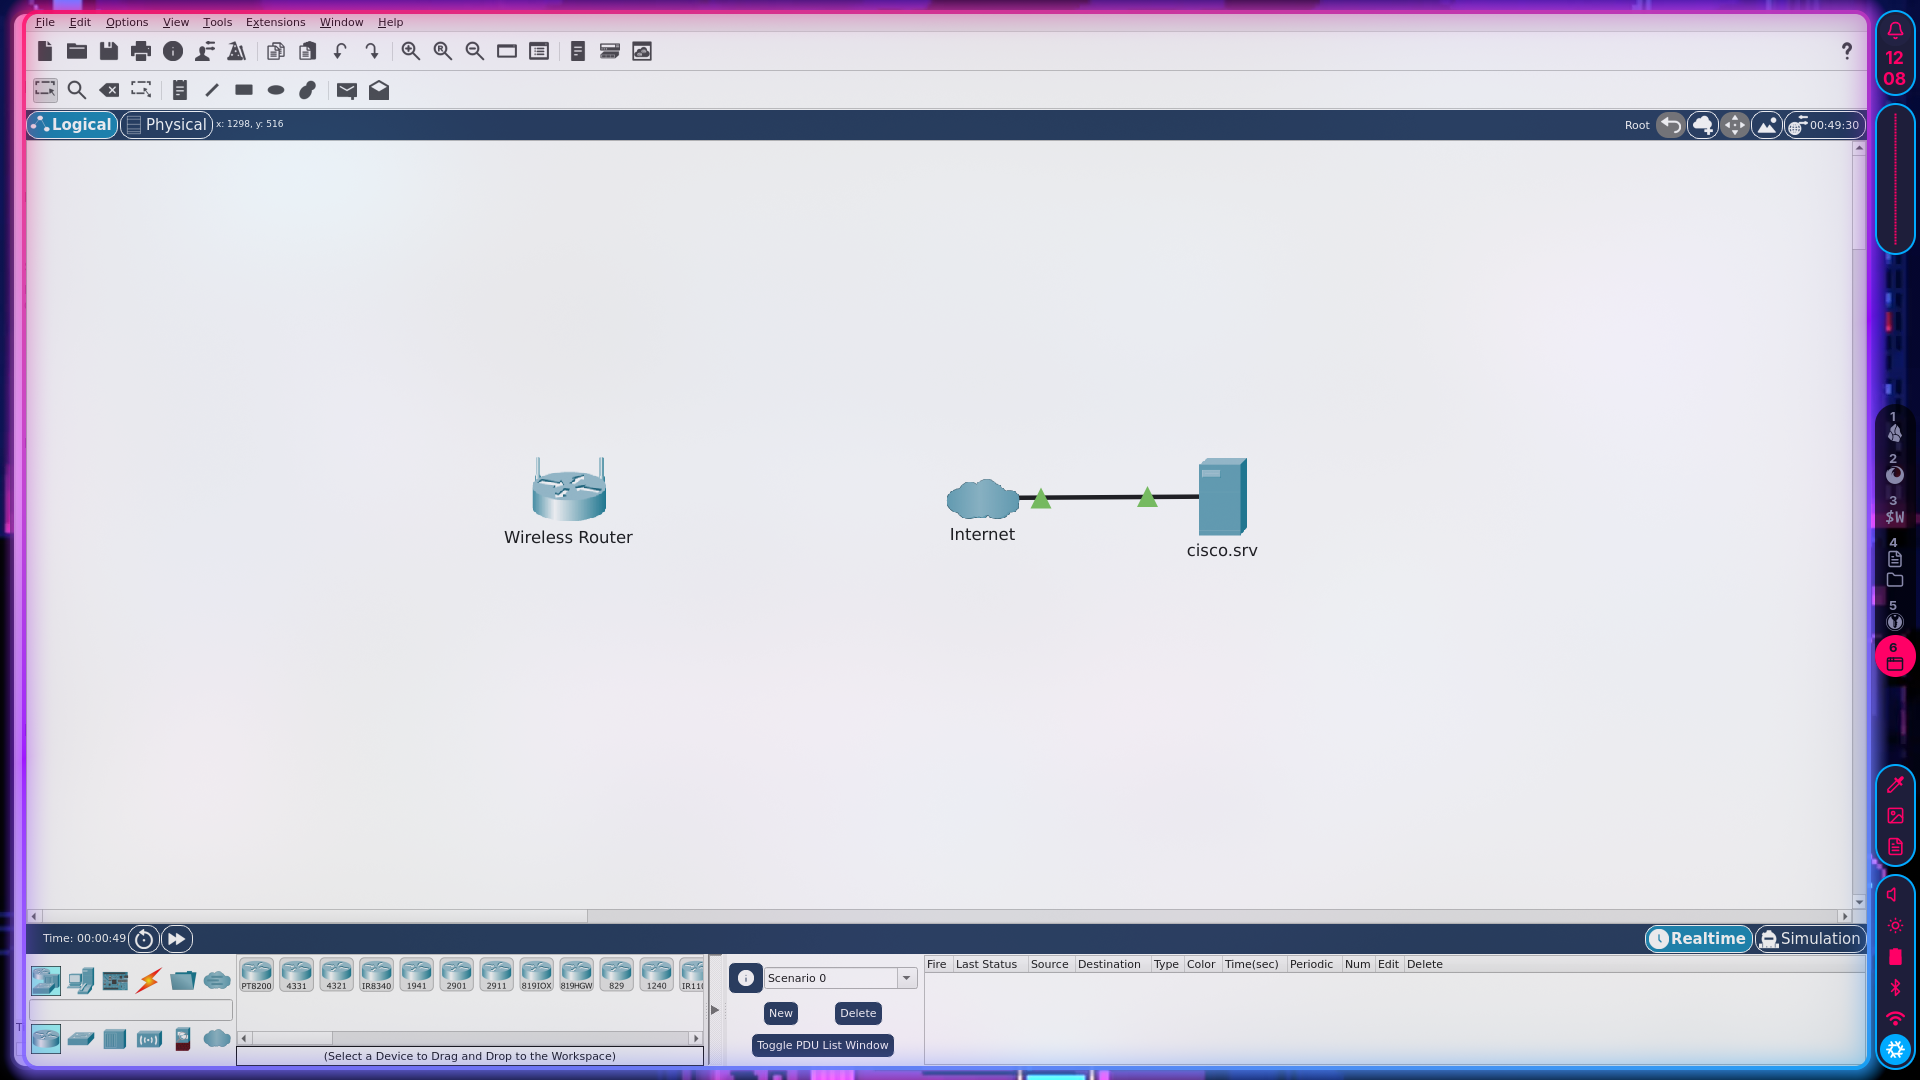
\includegraphics[width=0.85\textwidth]{../img/redSimple.png}
  \caption{Topología básica construida en el espacio lógico de Packet Tracer:
  router inalámbrico, nube de Internet y servidor conectados mediante enlaces
  de cobre operativos.}
  \label{fig:topologia}
\end{figure}

\begin{figure}[htbp]
  \centering
  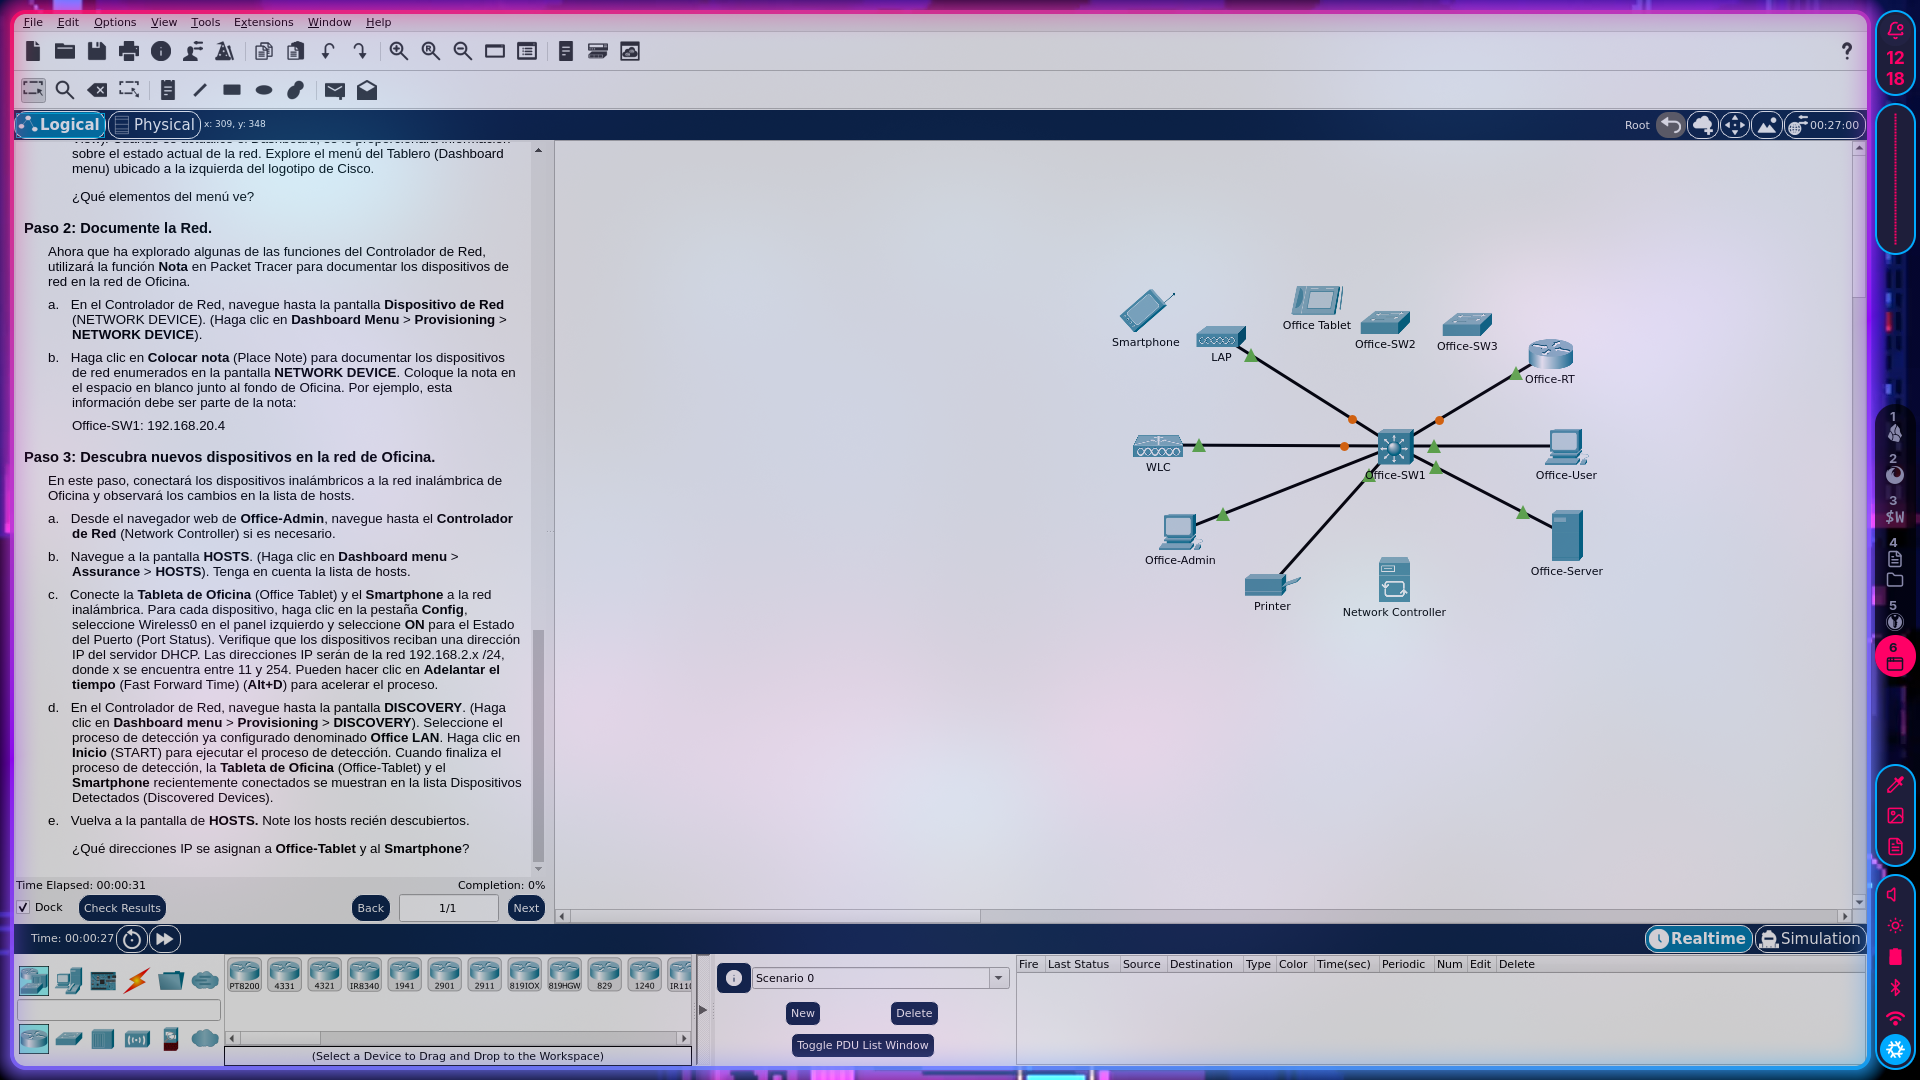
\includegraphics[width=0.85\textwidth]{../img/superviseRed.png}
  \caption{Red de oficina con switches de acceso y distribución, router,
  controlador inalámbrico, punto de acceso ligero y hosts cableados e
  inalámbricos con direccionamiento asignado por DHCP.}
  \label{fig:oficina}
\end{figure}

\subsection{Configuración y verificación mediante CLI}

La interfaz de línea de comandos se empleó tanto en la pestaña
\textit{Desktop} de los equipos finales como en la pestaña CLI de los
dispositivos de red. La Tabla~\ref{tab:cli} resume los comandos utilizados y su
propósito.

\begin{table}[htbp]
  \centering
  \small
  \begin{tabular}{@{}p{5.4cm}p{8.6cm}@{}}
    \toprule
    \textbf{Comando} & \textbf{Propósito} \\ \midrule
    \texttt{ipconfig /all} & Verificar dirección IP, máscara, puerta de enlace, MAC y servidores DHCP y DNS del host. \\
    \texttt{ping <destino>} & Comprobar conectividad de capa~3 y medir el tiempo de ida y vuelta. \\
    \texttt{tracert <destino>} & Conocer la ruta por saltos hasta el destino y localizar dónde se interrumpe. \\
    \texttt{nslookup <nombre>} & Resolver un nombre de dominio contra el servidor DNS. \\
    \texttt{enable} & Acceder al modo EXEC privilegiado del dispositivo. \\
    \texttt{configure terminal} & Entrar al modo de configuración global. \\
    \texttt{hostname <nombre>} & Asignar un nombre identificativo al dispositivo. \\
    \texttt{interface <if>} & Entrar al modo de configuración de una interfaz específica. \\
    \texttt{ip address <ip> <máscara>} & Asignar dirección IP y máscara a una interfaz. \\
    \texttt{no shutdown} & Habilitar administrativamente una interfaz. \\
    \texttt{show ip interface brief} & Resumir el estado y la dirección IP de todas las interfaces. \\
    \texttt{show running-config} & Mostrar la configuración activa en ejecución. \\
    \texttt{copy running-config startup-config} & Guardar la configuración para que persista tras reiniciar. \\ \bottomrule
  \end{tabular}
  \caption{Comandos de la CLI empleados en la configuración y verificación de
  los dispositivos de la red simulada.}
  \label{tab:cli}
\end{table}

La secuencia de configuración de una interfaz sigue un patrón constante: se
ingresa al modo de configuración global, se selecciona la interfaz, se asigna
la dirección y la máscara, se habilita con \texttt{no shutdown} y se verifica
el resultado con \texttt{show ip interface brief}. Los comandos de
verificación son tan importantes como los de configuración: permiten confirmar
que el cambio surtió efecto antes de continuar, en lugar de descubrir el error
al final del proceso.

\pendiente{captura de la sesión CLI mostrando \texttt{show ip interface brief}}

% ------------------ ANÁLISIS DEL FLUJO ----------------------
\section{Análisis del flujo de datos y de los protocolos}

El modo de simulación de Packet Tracer permite observar cada paquete como una
PDU que viaja entre dispositivos y detener el proceso para inspeccionar su
contenido capa por capa. El ejercicio más ilustrativo es el acceso a una página
web desde un equipo final recién conectado a la red. La secuencia observada es
la siguiente.

\begin{enumerate}[leftmargin=*]
  \item \textbf{Obtención de dirección (DHCP).} El equipo no tiene dirección
        IP, por lo que el cliente DHCP difunde \texttt{DHCPDISCOVER} en
        capa~2 con dirección MAC de destino de difusión. El servidor responde
        con \texttt{DHCPOFFER}, el cliente solicita con \texttt{DHCPREQUEST} y
        el servidor confirma con \texttt{DHCPACK}. A partir de ese momento el
        host conoce su IP, su máscara, la puerta de enlace y el servidor DNS.
  \item \textbf{Resolución de nombres (DNS).} El usuario escribe un nombre de
        dominio. Como la aplicación necesita una dirección IP, se genera una
        consulta DNS. Si el servidor DNS está fuera de la subred local, el
        paquete se dirige a la puerta de enlace; para enviarlo se requiere la
        MAC del router, lo que dispara el paso siguiente.
  \item \textbf{Resolución de direcciones (ARP).} El host emite una solicitud
        ARP difundida preguntando por la MAC de la puerta de enlace. El router
        responde con la suya y el host la almacena en su tabla ARP. Este mismo
        proceso ocurrirá en el router para el siguiente salto.
  \item \textbf{Establecimiento de la conexión (TCP).} Con la IP del servidor
        conocida, el cliente inicia el saludo de tres vías: \texttt{SYN} del
        cliente al servidor, \texttt{SYN-ACK} del servidor al cliente y
        \texttt{ACK} del cliente. La sesión queda establecida y lista para
        transportar datos de forma confiable.
  \item \textbf{Solicitud y respuesta (HTTP).} El cliente envía la petición
        \texttt{GET} al puerto~80 (o~443 si es HTTPS, con cifrado TLS
        previo). El servidor responde con el contenido solicitado, que se
        segmenta, se numera y se confirma.
\end{enumerate}

\paragraph{Encapsulación y desencapsulación.} En cada uno de estos pasos la
información desciende por las capas del emisor y asciende por las del
receptor. La aplicación genera los datos; la capa de transporte los segmenta y
agrega puertos de origen y destino; la capa de red añade las direcciones IP,
formando el paquete; la capa de enlace construye la trama con las direcciones
MAC del enlace local; y la capa física convierte todo en señales que viajan por
el medio. En el destino el proceso se invierte.

\paragraph{Qué cambia y qué permanece.} La observación más valiosa del ejercicio
es que, a lo largo de toda la ruta, \textbf{las direcciones IP de origen y
destino permanecen constantes} —son el identificador extremo a extremo—,
mientras que \textbf{las direcciones MAC se reescriben en cada salto}, porque
identifican únicamente el enlace local. Si hay NAT de por medio, la dirección
IP privada de origen se sustituye por la pública y el puerto se reasigna, pero
la IP de destino se conserva.

\paragraph{Correspondencia con los modelos.} Este recorrido hace tangible la
relación entre OSI y TCP/IP. DHCP, DNS y HTTP operan en la capa de aplicación;
TCP y UDP en la de transporte; IP y ARP en la de red —ARP técnicamente en el
límite entre red y enlace, pues resuelve direcciones de enlace a partir de
direcciones lógicas—; Ethernet en la de enlace; y el medio en la física. Un
fallo en cualquiera de estos pasos interrumpe el acceso web, y la utilidad de
diagnóstico adecuada depende de identificar en cuál ocurrió. Esa es la razón
por la que el modelo OSI sigue siendo una herramienta práctica y no solo un
esquema teórico.

\pendiente{captura del panel de simulación con la PDU y el detalle por capas}

% --------------------- SÍNTESIS REFLEXIVA -------------------
\section{Síntesis reflexiva de competencias adquiridas}

Completar \textit{Conceptos Básicos de Redes} produjo un cambio en la forma de
entender el funcionamiento de una red: de una colección de dispositivos
conectados a un sistema jerárquico donde cada capa resuelve un problema
específico y delega el resto.

En el plano conceptual, el aprendizaje más sólido fue la separación de
responsabilidades entre capas. Comprender que la capa de red se ocupa del
direccionamiento lógico extremo a extremo mientras la de enlace se ocupa de la
entrega en el tramo local explica hechos que de otro modo parecen arbitrarios,
como que las MAC cambien en cada salto mientras las IP se conservan. Ese
principio ordena el diagnóstico: ante una falla, la pregunta deja de ser
``no hay Internet'' y se convierte en ``¿en qué capa se rompió la cadena?''.

En el plano instrumental, el curso consolidó el uso de Packet Tracer como
laboratorio: construir topologías, configurar interfaces por CLI, verificar el
estado con comandos y detener la simulación para inspeccionar una PDU. La
posibilidad de observar el paquete detenido, abrir su cabecera y comprobar qué
campos cambian respecto del salto anterior convierte la encapsulación en algo
verificable en lugar de memorizable.

En el plano metodológico, quedó instalada una disciplina de verificación
ascendente: configuración local, conectividad con la puerta de enlace,
conectividad externa y resolución de nombres. Es un procedimiento reproducible
que evita el ensayo y error, y que se transfiere directamente al trabajo con
equipos reales.

Finalmente, el curso dejó clara la razón por la que IPv6 y NAT existen: detrás
de decisiones técnicas aparentemente simples hay límites de diseño —el
agotamiento del espacio de 32 bits— que obligaron a introducir soluciones de
compromiso. Entender ese contexto histórico hace que el direccionamiento deje
de ser un conjunto de reglas y se vuelva una consecuencia lógica.

% -------------------------- CONCLUSIÓN ----------------------
\section{Conclusión}

Se completó el curso \textit{Conceptos Básicos de Redes} de Cisco Networking
Academy, cubriendo los diecisiete módulos que lo integran y aprobando los
exámenes de punto de control y el examen final correspondientes. Como
evidencia de finalización se anexan la constancia del progreso al 100\,\% y el
certificado emitido por la plataforma (Anexo~A).

Los objetivos planteados se cumplieron: se describieron los modelos OSI y
TCP/IP y la función de cada capa; se distinguieron los tipos de red y los
dispositivos que intervienen en cada uno; se identificaron los medios de
transmisión y sus criterios de selección; se aplicó el direccionamiento IPv4 e
IPv6, incluida la segmentación y la asignación dinámica por DHCP; se explicó el
proceso ARP y el reenvío entre redes; se compararon TCP y UDP; y se emplearon
las utilidades de prueba de red dentro de un procedimiento de diagnóstico
ordenado.

El resultado es una base conceptual sólida sobre la que la materia de Redes de
Comunicaciones de Datos puede construir los temas de enrutamiento, conmutación
y diseño de infraestructuras de mayor complejidad, y la confirmación de que la
comprensión del flujo de datos a través de las capas es la herramienta de
diagnóstico más útil que puede adquirirse en esta etapa de la formación.

% --------------------------- ANEXO --------------------------
\appendix

\section{Anexo A: Constancia de finalización}

\subsection{Progreso del curso al 100\,\%}

% TODO: captura de la pantalla de NetAcad con el progreso general al 100 %
% (Course Outline, todas las barras en verde, y el certificado visible).
\pendiente{captura del progreso al 100\,\% en NetAcad}

\subsection{Certificado de finalización}

% TODO: descargar el certificado en PDF desde NetAcad
% (Home > My Learning > Conceptos Básicos de Redes > Certificate)
% y guardarlo en esta carpeta como certificado.pdf
\pendiente{archivo certificado.pdf del curso}

% Cuando el PDF exista, habilitar la línea siguiente:
% 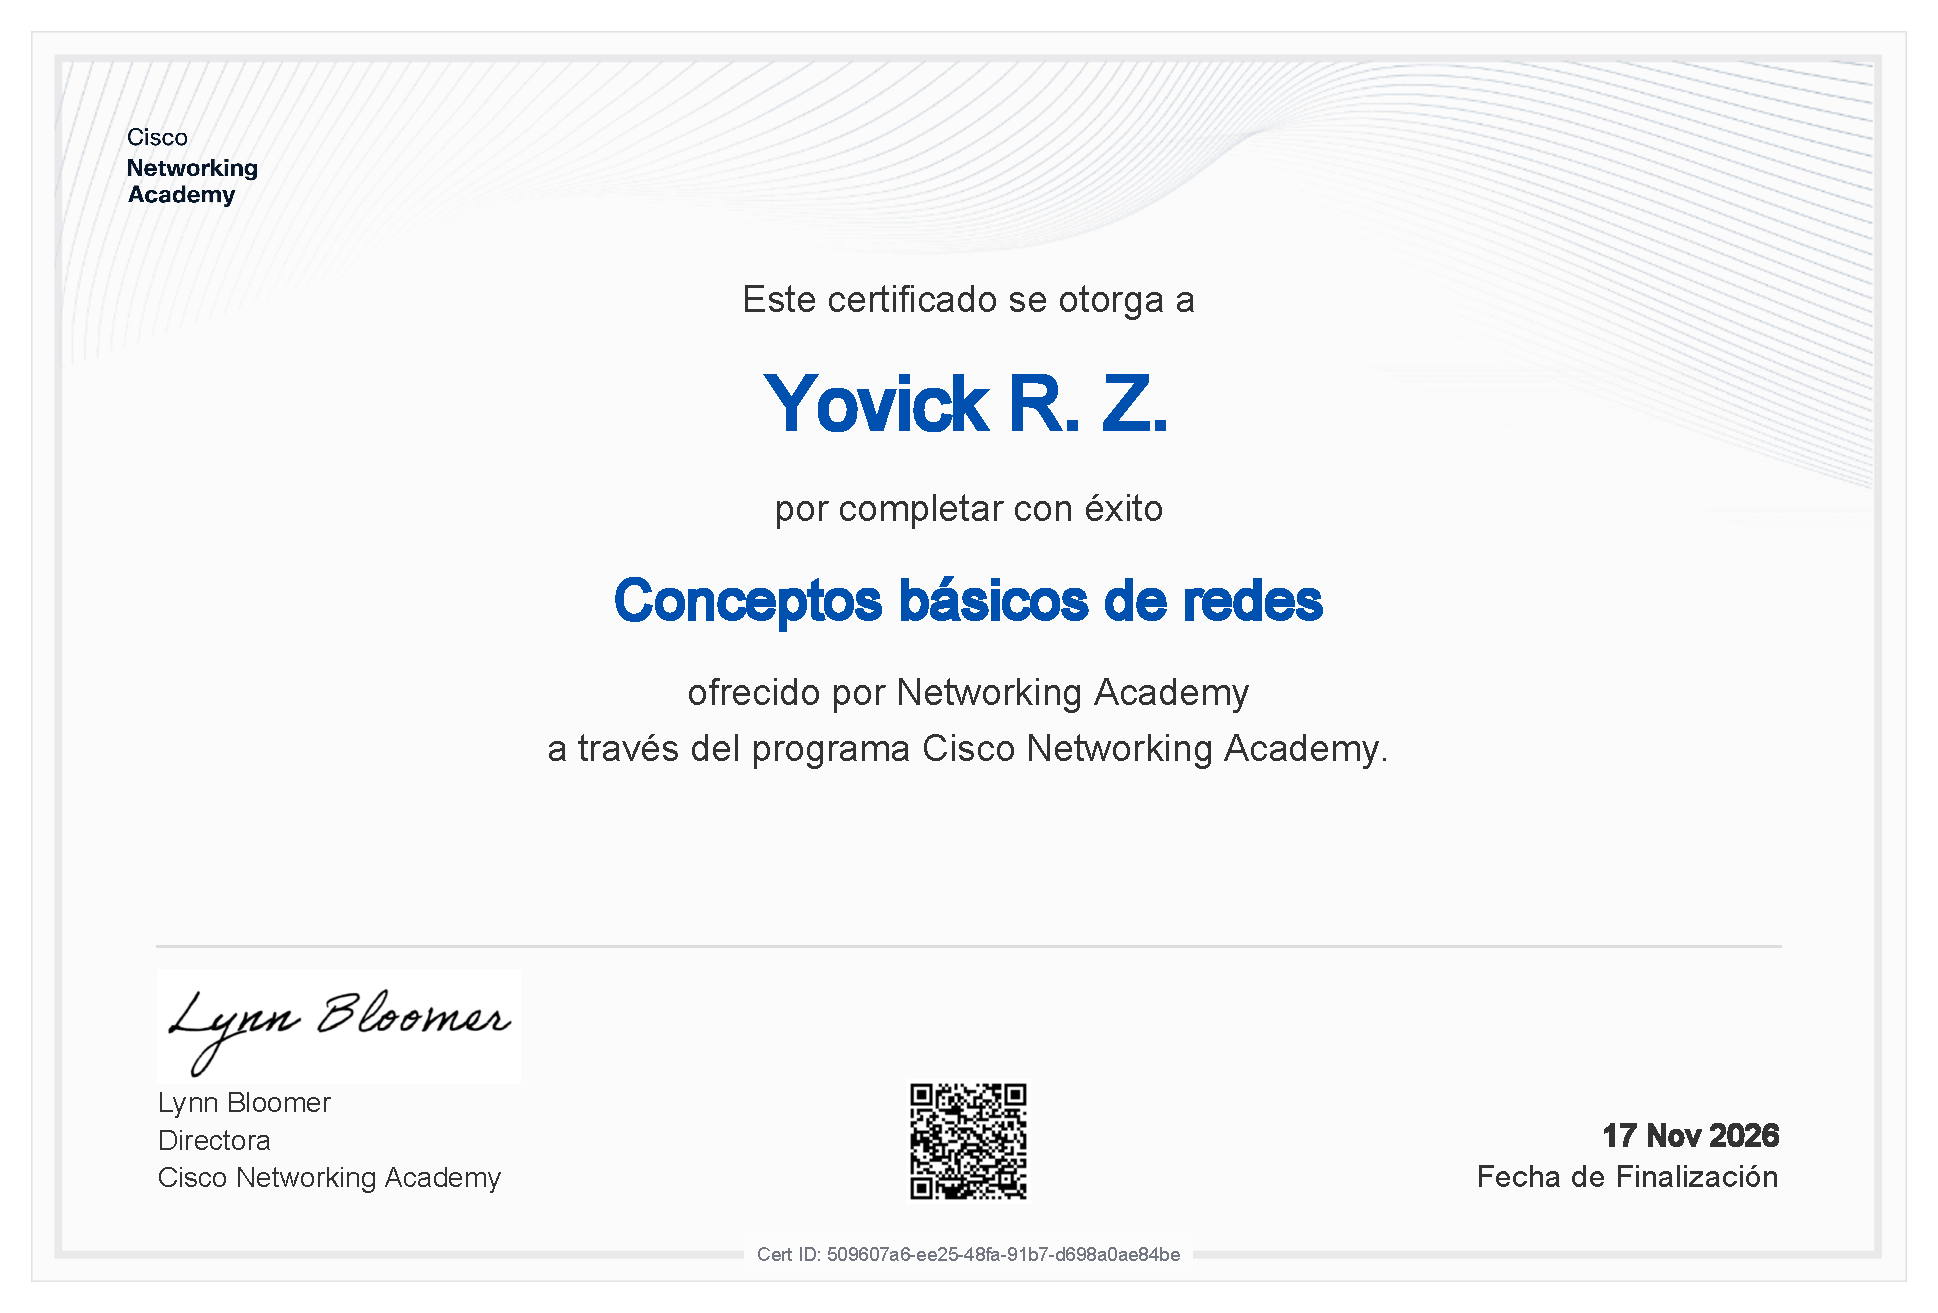
\includepdf[pages=-,pagecommand={\thispagestyle{fancy}}]{certificado.pdf}

\section{Anexo B: Evidencias de las prácticas en Packet Tracer}

% TODO: capturas adicionales de cada actividad del curso
\pendiente{capturas de las actividades de Packet Tracer}

\end{document}
